
\documentclass{article}
\usepackage[utf8]{inputenc}
\usepackage{graphicx}
\graphicspath{{figures/}}
\usepackage{caption}
\usepackage{subcaption}
\usepackage{amsmath}
\usepackage{booktabs}
\usepackage{float}     % gives [H] exact placement
\usepackage{placeins}  % gives \FloatBarrier to stop floats crossing
\usepackage{geometry}
\geometry{margin=1in}
\title{Model Performance and Feature Analysis: A Pipeline Approach}
\author{}
\date{}

\begin{document}

\maketitle

\section{Introduction}

This project focuses on forecasting soil moisture content (SWC) using a variety of machine learning models. I developed a modular forecasting pipeline to evaluate model performance across different temporal configurations and soil depths. The models tested include convolutional neural networks (CNNs), long short-term memory networks (LSTMs), ARIMA, and XGBoost.

The pipeline supports varying input/output window sizes, feature engineering and filtering, seasonal testing splits, hyperparameter tuning, and manual and automatic feature selection.

I consistently evaluated performance using Mean Absolute Error (MAE). Experiments were conducted for 10 cm SWC, using hourly meteorological and soil measurements from multiple stations in Texas. Models were tested for performance with 48 hour, 72 hour, and 168 hour prediction targets. I also tested performance by season, and also attempted testing the affect of manual hyperparameter tuning on these large models, as is standard practice with simpler ML models through techniques like GridSearchCV. At the end, I presented some results from my feature importance investigation with these various models.

\section{Dataset}
I used hourly meteorological and soil data from six stations in Texas. The dataset includes:
\begin{itemize}
    \item Target variables: SWC at 5, 10, 20, and 50 cm depths (\texttt{SWC\_5}, \texttt{SWC\_10}, etc.).
    \item Environmental features: Soil temperature at multiple depths (T\_5, T\_10, ..., T\_50), precipitation (Ppt), relative humidity (RH), air temperature (Tair), solar radiation (Srad), wind speed, wind direction.
    \item Time encodings.
    \item Location Data (Latitude/Longitude)
\end{itemize}
Missing values and anomalies have been previously addressed and were not a concern, as this project was built on a cleaned dataset. Location data was excluded to avoid unnecessary/extraneous complexity.

\section{Feature Filtering and Engineering}

\subsection{Feature Filtering}

To streamline model input and reduce noise, we applied both manual feature selection and optional correlation-based filtering.

\paragraph{Manual Selection:}
\begin{itemize}
    \item Many features are collected at multiple depths (e.g., \texttt{SWC\_5}, \texttt{SWC\_10}, \texttt{SWC\_20}, \texttt{T\_5}, \texttt{T\_50}).
    \item We retained:
    \begin{itemize}
        \item \texttt{SWC\_10} - as the primary prediction target.
        \item \texttt{T\_5} - due to strong correlation and consistent model performance.
    \end{itemize}
\end{itemize}

\paragraph{Automated Correlation Filtering (Optional):}
\begin{itemize}
    \item A correlation matrix is computed for all numeric features not manually retained.
    \item Features with pairwise correlation above a set threshold are flagged.
    \item In each pair, one feature is dropped to prevent multicollinearity and redundancy.
    \item This reduces input complexity and helps mitigate overfitting.
\end{itemize}

\paragraph{Final Selection:}
\begin{itemize}
    \item Core features: \texttt{SWC\_10}, \texttt{T\_5}
    \item Optional additions based on analysis:
    \begin{itemize}
        \item \texttt{RH}, \texttt{Srad}, \texttt{Ppt}, \texttt{Wind\_X}, \texttt{Wind\_Y}
    \end{itemize}
    \item These were selected based on exploratory analysis (\texttt{data\_analysis.ipynb}).
    \item Most tests were run using only \texttt{SWC\_10} and \texttt{T\_5}.
    \item In the \textit{Feature Importance} section, we explore the impact of adding more features.
\end{itemize}

\subsection{Feature Engineering}

\begin{itemize}
    \item \textbf{Wind Vectors:} \texttt{Wind\_X} and \texttt{Wind\_Y} are Cartesian transformations of \texttt{Windspeed} and \texttt{Winddirection}, capturing wind velocity as a vector.
    \item \textbf{Temporal Cyclical Features:} \texttt{DaySin}, \texttt{DayCos}, \texttt{YearSin}, \texttt{YearCos} encode seasonality in a continuous, periodic manner using sine and cosine transformations. These features preserve cyclicity and scale values between 0 and 1.
\end{itemize}


\section{Data Windowing and Normalization}

The following preprocessing steps are applied to models that require time-series batching and scale-sensitive input representations, specifically CNN, LSTM, Bi-LSTM, and XGBoost. Neural networks in particular are sensitive to input distributions and benefit from windowed inputs.

\subsection{Data Windowing}

Time series data was transformed into overlapping input-output sequences to enable supervised learning.

\begin{itemize}
    \item Each input window represents a fixed-length segment of historical data (72 hours of hourly data).
    \item The model is trained to predict a future target at a fixed offset from the end of the window.
    \item We evaluated three prediction horizons:
    \begin{itemize}
        \item 48-hour forecast
        \item 72-hour forecast
        \item 168-hour forecast
    \end{itemize}
    \item This process enables multi-step forecasting and generates a large training set from continuous time series data.
\end{itemize}

\subsection{Data Normalization}

\begin{itemize}
    \item All features were scaled using \texttt{StandardScaler} to have zero mean and unit variance.
    \item The transformation was fit on the training data and applied to both train and test splits.
    \item During model evaluation, only the target variable (\texttt{SWC\_10}) was inverse-transformed to recover predictions in physical units (soil moisture percentage).
    \item This ensures comparability across models and accurate interpretation of results.
\end{itemize}


\section{Modeling}

\subsection{ARIMA (Autoregressive Integrated Moving Average)}
ARIMA is a traditional statistical model suited for univariate time series. It was used as a baseline in our experiments. Since ARIMA cannot utilize exogenous inputs by default, it generally underperformed compared to more complex models. It was most effective in winter, when soil moisture patterns were stable since rain was little, but failed to capture multivariate and non-linear dependencies in other seasons. It achieved its best performance in more stable conditions but struggled to capture multivariate dependencies, leading to the highest RMSE overall.

\subsection{ARIMAX (ARIMA with Exogenous Inputs)}
ARIMAX extends ARIMA by incorporating exogenous variables, enabling it to use additional predictors such as temperature, rainfall, and radiation. This provided it with more contextual information than ARIMA alone, improving performance slightly better than ARIMA, but still trailing behind modern ML models. Its linear nature limited its ability to handle complex feature interactions, leading to a relatively high RMSE.

\subsection{LSTM (Long Short-Term Memory Networks)}
LSTM is a deep learning model designed for sequence data. It was implemented using Keras, with parameters like number of units, activation function, and dropout rate set manually or through tuning. LSTM performed well in seasons with consistent temporal patterns (especially winter), but its performance degraded a bit in noisier seasons like summer. It showed a strong ability to model long-term dependencies, but was sensitive to hyperparameters and required normalization and careful windowing.

\subsection{BiLSTM (Bidirectional Long Short-Term Memory)}
BiLSTM processes time series in both forward and backward directions, enabling it to learn from both past and future context within a training window. This gave it an edge over standard LSTM in capturing symmetrical dependencies, making it the second-best performer in terms of RMSE. BiLSTM was especially effective when short-term fluctuations influenced outcomes as well as long-term ones. Its strong performance suggests that bidirectional context is valuable for soil moisture forecasting, as well as forecasting complex time series data in general.

\subsection{CNN (Convolutional Neural Network)}
CNNs were used with 1D convolutions to extract temporal features over short windows. While CNNs performed well in stable conditions (winter), their performance dropped in seasons with more variability. CNNs require careful design of filter sizes and dropout to prevent overfitting. Unlike LSTM or BiLSTM, CNN models are more local in focus and may miss long-range dependencies.

\subsection{XGBoost (Extreme Gradient Boosting)}
XGBoost consistently delivered strong performance across all seasons. It is robust to outliers, can handle non-linear patterns, and performs well without needing heavy data preprocessing. By flattening the input window into a 2D array, XGBoost was able to capture relationships across time steps effectively. It outperformed all other models in terms of both accuracy and consistency, with low RMSE, MAE, and MAPE across the board.


\begin{figure}[H]
    \centering
    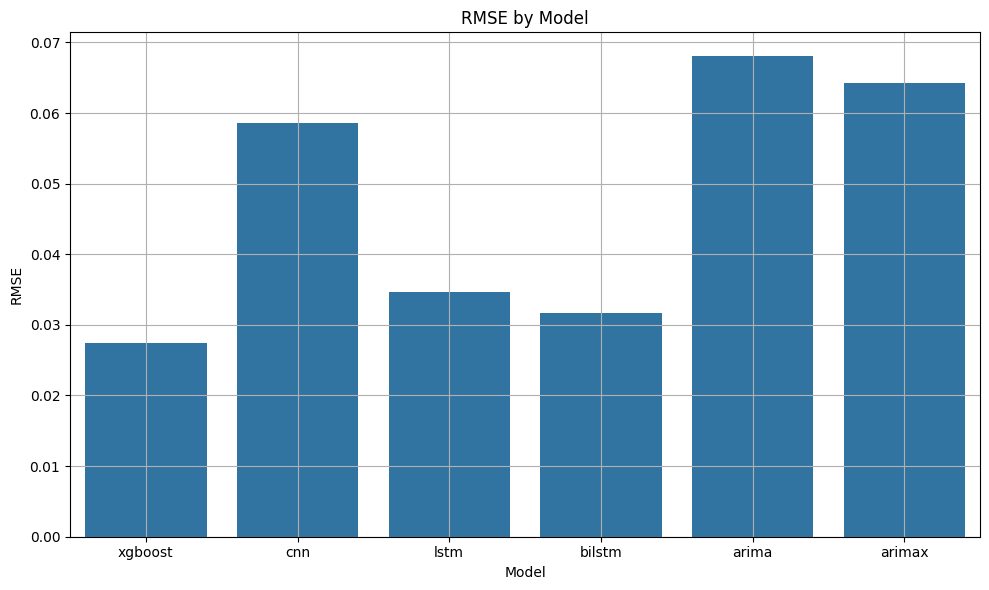
\includegraphics[width=\linewidth]{rmse_all.png}
    \caption{Overall RMSE comparison across models aggregated over all seasons and horizons.}
    \label{fig:rmse-overall}
\end{figure}



\section{Seasonal Performance}

Model performance varies noticeably across seasons. All models perform best in winter, likely due to little rain and more steady weather patterns. In contrast, summer and fall are more challenging due to complex interactions of precipitation and heat. Among the models, XGBoost demonstrates strong and stable performance across all seasons, while BiLSTM also delivers consistently strong results, especially in more variable conditions. LSTM performs well but is more sensitive to seasonal fluctuations that are difficult to capture. CNNs show good winter performance but suffer more in irregular conditions. ARIMA consistently lags behind due to its linear, univariate nature, while ARIMAX benefits from exogenous features and performs a bit better than ARIMA.

\begin{figure}[H]
    \centering
    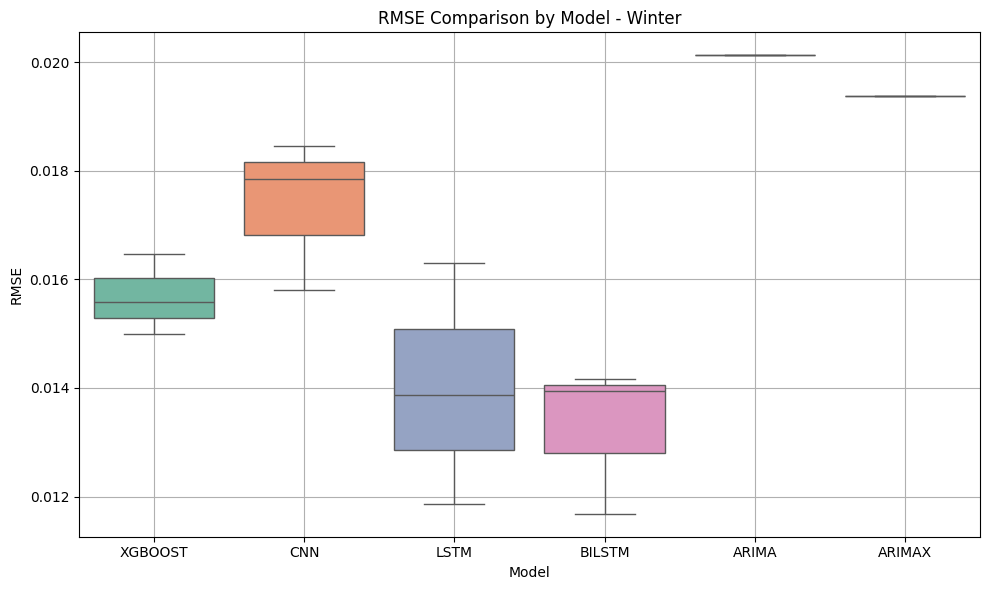
\includegraphics[width=\linewidth]{season_winter.png}
    \caption{Seasonal model performance (RMSE) - Winter.}
    \label{fig:season-winter}
\end{figure}

\begin{figure}[H]
    \centering
    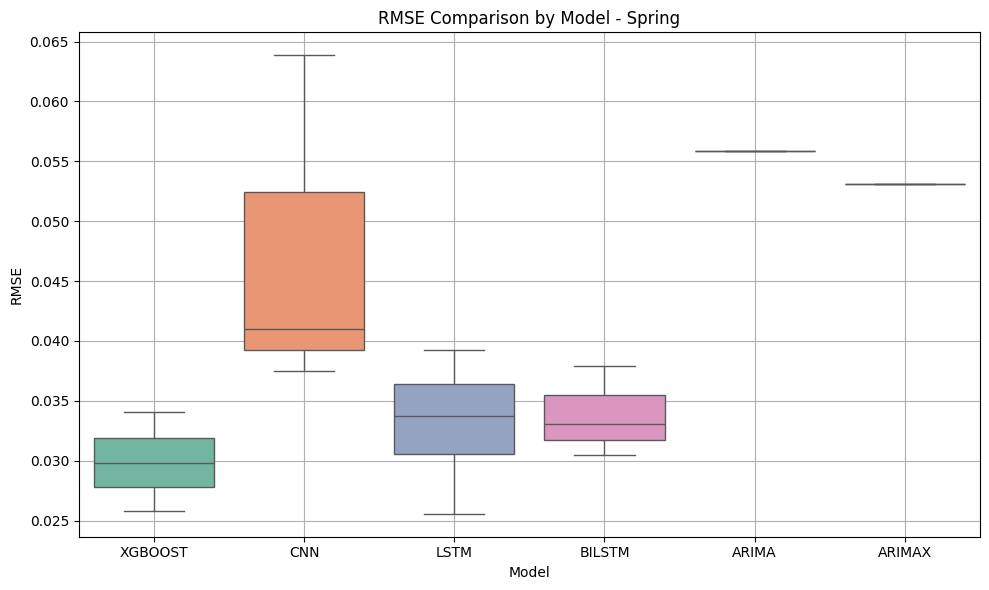
\includegraphics[width=\linewidth]{season_spring.png}
    \caption{Seasonal model performance (RMSE) - Spring.}
    \label{fig:season-spring}
\end{figure}

\begin{figure}[H]
    \centering
    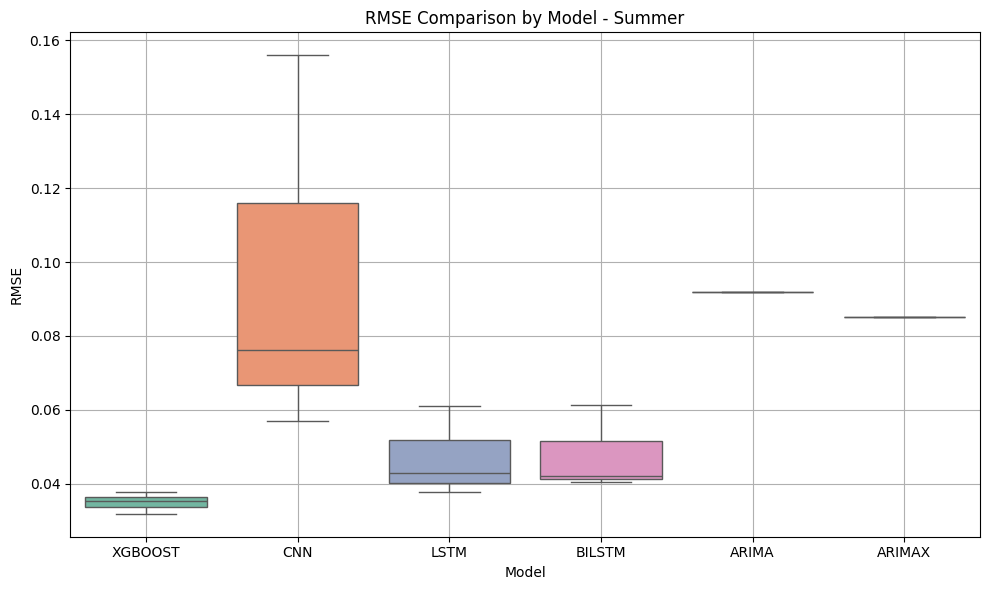
\includegraphics[width=\linewidth]{season_summer.png}
    \caption{Seasonal model performance (RMSE) - Summer.}
    \label{fig:season-summer}
\end{figure}

\begin{figure}[H]
    \centering
    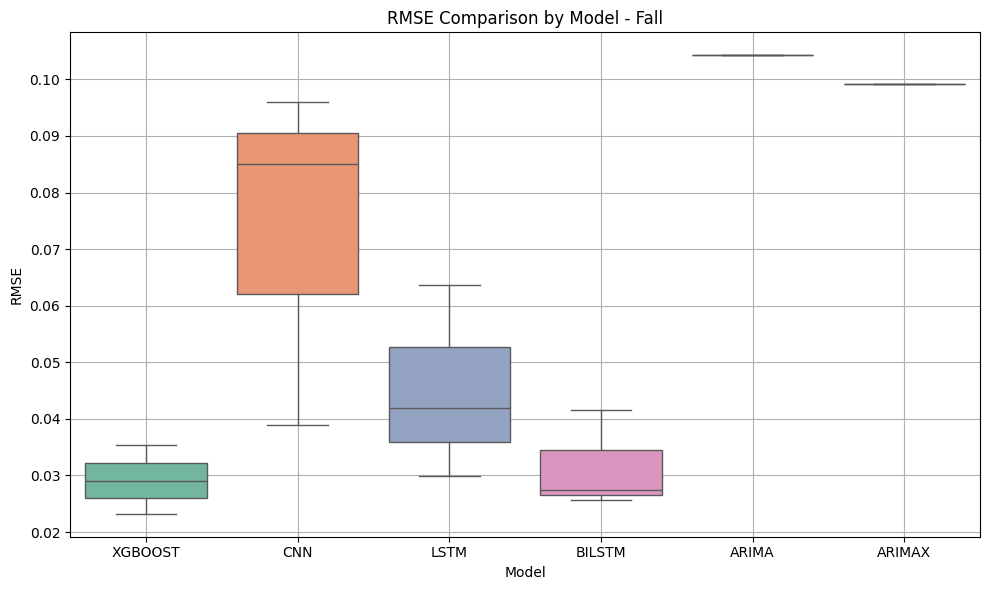
\includegraphics[width=\linewidth]{season_fall.png}
    \caption{Seasonal model performance (RMSE) - Fall.}
    \label{fig:season-fall}
\end{figure}


\subsection{Winter}
\begin{itemize}
    \item All models performed best in winter, which had the lowest average RMSE and MAPE.
    \item Patterns were more consistent due to lower precipitation variability.
    \item ARIMA and ARIMAX, despite being linear, performed relatively well, with ARIMAX outperforming ARIMA due to additional predictors.
    \item XGBoost and BiLSTM achieved the best scores across all metrics, with LSTM close behind.
\end{itemize}

\subsection{Spring}
\begin{itemize}
    \item Performance began to diverge across models due to increased variance.
    \item CNN and LSTM remained effective but started showing more error spread.
    \item BiLSTM maintained strong performance, showing better handling of variance.
    \item ARIMAX generally outperformed ARIMA.
    \item XGBoost remained stable and continued outperforming others.
\end{itemize}

\subsection{Summer}
\begin{itemize}
    \item This was the most challenging season, with highly variable weather and soil moisture due to rainfall and heat.
    \item All models showed increased RMSE and MAPE.
    \item LSTM and CNN had significantly lower correlation, indicating poor trend capturing.
    \item BiLSTM performed better than LSTM, benefiting from bidirectional context.
    \item ARIMAX also struggled with capturing complex patterns.
    \item XGBoost maintained reasonable error rates and high correlation, outperforming others.
    \item ARIMA performed the worst, showing its limitations with non-stationary data.
\end{itemize}

\subsection{Fall}
\begin{itemize}
    \item Similar to summer, with high variance and lower correlation in LSTM and CNN.
    \item BiLSTM again proved more robust than LSTM, ranking among the top two models.
    \item ARIMA showed its worst performance in fall across all metrics.
    \item XGBoost again remained consistent, highlighting its robustness.
\end{itemize}

\section{Varying Offset Performance}

All models showed increasing RMSE with longer horizons, reflecting the logical growing uncertainty with longer-term predictions. 

\begin{figure}[H]
    \centering
    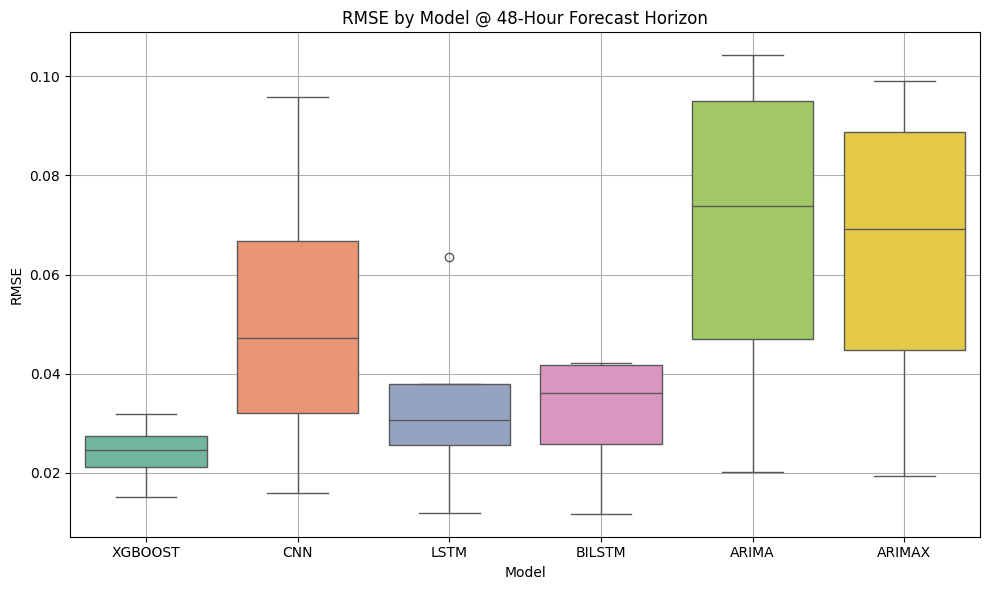
\includegraphics[width=\linewidth]{horizon_48.png}
    \caption{RMSE by model at 48-hour forecast horizon.}
    \label{fig:horizon-48}
\end{figure}

\begin{figure}[H]
    \centering
    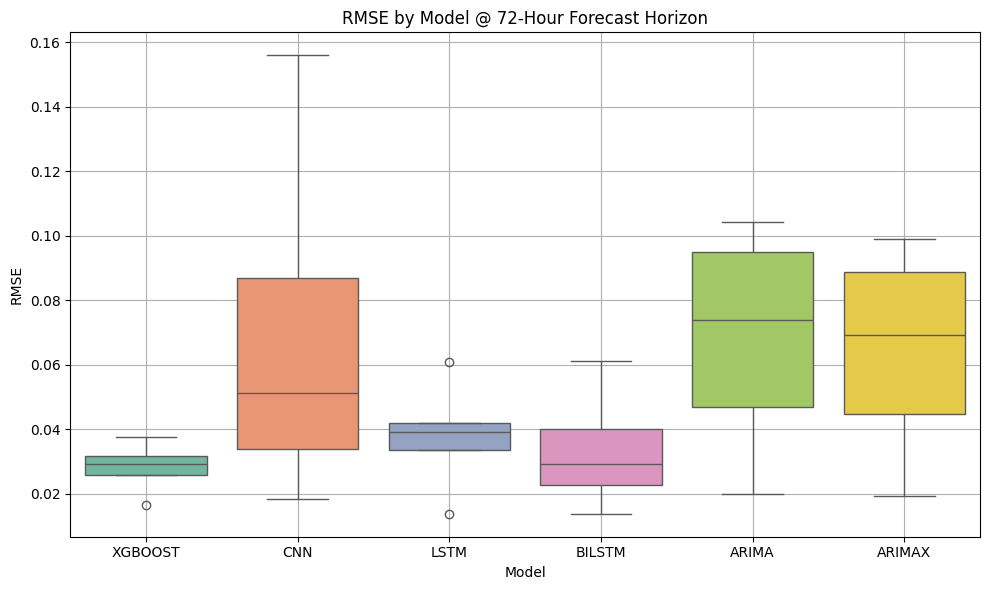
\includegraphics[width=\linewidth]{horizon_72.png}
    \caption{RMSE by model at 72-hour forecast horizon.}
    \label{fig:horizon-72}
\end{figure}

\begin{figure}[H]
    \centering
    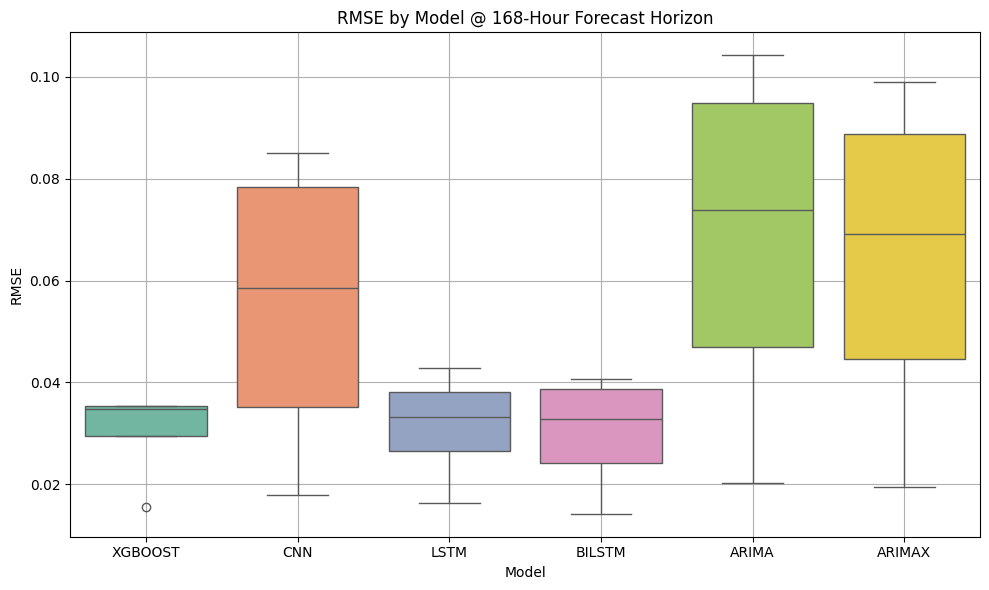
\includegraphics[width=\linewidth]{horizon_168.png}
    \caption{RMSE by model at 168-hour forecast horizon.}
    \label{fig:horizon-168}
\end{figure}



\begin{itemize}
    \item \textbf{XGBoost} maintained the most stable RMSE, with relatively small increases even at 168 hours. This demonstrates its robustness in multi-step forecasting.
    \item \textbf{LSTM} and \textbf{BiLSTM} consistently ranked among the top performers at every horizon. Their RMSE barely rose with forecast length, showing the effectiveness of memory-based capturing of temporal patterns.
    \item \textbf{ARIMA} and \textbf{ARIMAX} performed poorly across all horizons, with the highest RMSEs and the most degradation from 48 hours to 168 hours. Their performance decline confirms their limitations due to a linear nature and difficulty handling compounding uncertainty.
\end{itemize}

\section{Feature Set Analysis}
To evaluate the influence of different input feature combinations on model performance, we designed controlled experiments where each forecasting model was trained and tested on multiple subsets of available variables.

The feature subsets ranged from:
\begin{itemize}
    \item \textbf{Minimal set:} Only \texttt{SWC\_10} and \texttt{T\_5}.
    \item \textbf{Intermediate set:} Core soil and temperature features plus \texttt{RH}, \texttt{Srad}, and \texttt{Ppt}.
    \item \textbf{Full set:} All above plus \texttt{Wind\_X}, \texttt{Wind\_Y}, and cyclical time encodings (\texttt{DaySin}, \texttt{DayCos}, \texttt{YearSin}, \texttt{YearCos}).
\end{itemize}

This approach isolated the effect of feature composition while holding all other variables constant. The pipeline steps were identical to the main experiments. Due to time constraints, the full impact of each feature was not properly assessed, as tests were not extensive, but here's a general analysis: 

For CNN and LSTM models, the full set of meteorological and seasonal features produced the lowest RMSE and MAPE values, particularly for shorter horizons. On the contrary, XGBoost proved resilient to feature reductions but still benefited from the additional context. Neural networks, especially BiLSTM, leveraged richer inputs to capture more complex temporal relationships, yielding the highest correlations and lowest errors.


\section{Results}

\subsection{Overall Model Performance}
Across all seasons and horizons(Figure~\ref{fig:rmse-overall}), XGBoost achieved the lowest aggregate RMSE, closely followed by BiLSTM. LSTM and CNN formed the middle tier, while ARIMAX and ARIMA consistently trailed behind. The ranking was consistent across both error magnitude and stability, proving how model choice directly impacts predictive accuracy in soil moisture forecasting.

\subsection{Seasonal Analysis}
Model performance varied noticeably from season to season (Figures~\ref{fig:season-winter}--\ref{fig:season-fall}).  
In \textbf{winter} (Figure~\ref{fig:season-winter}), all models delivered their strongest results. The stable, low-variability conditions favored even the simpler statistical approaches, with ARIMAX edging out ARIMA thanks to its additional predictors. XGBoost and BiLSTM led the pack, with LSTM performing closely behind.  
In \textbf{spring} (Figure~\ref{fig:season-spring}), increasing variability began to separate the models. XGBoost continued to lead, while BiLSTM maintained strong, consistent performance. CNN and LSTM remained competitive but showed more spread in their errors, and ARIMAX maintained a small advantage over ARIMA.  
In \textbf{summer} (Figure~\ref{fig:season-summer}), high variability from heat and rainfall created a tougher prediction environment. All models saw higher errors, but the drop in correlation for LSTM and CNN was especially sharp. BiLSTM proved more resilient, while ARIMAX struggled alongside ARIMA. XGBoost handled the conditions best, with only a modest increase in error.  
In \textbf{fall} (Figure~\ref{fig:season-fall}), the challenges looked similar to summer. XGBoost again remained steady, BiLSTM continued to outperform LSTM, and ARIMA recorded its weakest seasonal performance.

\subsection{Horizon Analysis}
As expected, forecast accuracy declined as the prediction horizon increased (Figures~\ref{fig:horizon-48}--\ref{fig:horizon-168}).  
At \textbf{48 hours} (Figure~\ref{fig:horizon-48}), XGBoost, BiLSTM, and LSTM, produced similarly competitive results, showing strong short-term forecasting ability.  
At \textbf{72 hours} (Figure~\ref{fig:horizon-72}), the performance gap widened, with XGBoost pulling ahead and BiLSTM holding a clear second place.  
At \textbf{168 hours} (Figure~\ref{fig:horizon-168}), the differences became more pronounced. XGBoost’s error rose only modestly, highlighting its robustness for long-range forecasts. LSTM’s accuracy dropped more sharply than BiLSTM’s, underscoring the benefit of bidirectional context. ARIMA and ARIMAX saw the steepest declines, reaffirming the limitations of these linear models when dealing with compounding uncertainty over extended horizons.

\subsection{Impact of Feature Sets}
Across all models, richer feature sets improved predictive accuracy, though the degree of improvement varied:
\begin{itemize}
    \item \textbf{BiLSTM and LSTM} benefited the most from expanded features, showing substantial RMSE reductions when meteorological and temporal context was added.
    \item \textbf{XGBoost} delivered strong results even with minimal features, but still gained moderate accuracy improvements with the full feature set.
    \item \textbf{CNN} performance increased significantly with richer inputs, indicating its advantage in extracting local temporal patterns from multivariate data.
    \item Minimal feature configurations led to notable accuracy drops for deep learning models, emphasizing the value of diverse feature inputs.
\end{itemize}


\section{Conclusion}
This study highlights how model choice, feature selection, and forecast horizon affect soil moisture prediction accuracy. Among all approaches tested, XGBoost stood out as the most reliable and accurate, even under highly variable conditions. BiLSTM followed closely, showing particular strength in complex seasonal patterns and long-term forecasts. LSTM also performed well for shorter horizons but proved more sensitive to changes in seasonality and forecast length.

ARIMAX, while a clear improvement over baseline ARIMA due to exogenous features, remained bottle-necked by its linear design. Both ARIMAX and ARIMA struggled to maintain accuracy in longer-range and more variable conditions. CNNs proved effective at capturing stable, local patterns but lacked the ability to model long-term data, making them less competitive in our analysis.

Overall, the results suggest that XGBoost and BiLSTM are strong candidates for soil moisture forecasting. Future work with this data and pipeline could explore hybrid models that combine the feature extraction capabilities of deep learning with the structured decision-making of ensemble methods, as well as adaptive systems that adjust the model choice dynamically based on seasonal conditions or prediction window. With more computing power, the idea of tuning these large models like small ones could be explored as well. Overall, the optimization problem never ends, but here my contribution to it concludes. Thanks for looking into my work.

\end{document}
